\documentclass{article}
\usepackage[utf8]{inputenc}
\usepackage[portuguese]{babel}
\usepackage{csquotes}
\usepackage{graphicx}
\usepackage{adjustbox}
\usepackage{lipsum}
\usepackage[backend=biber,autolang=other,
  bibencoding=utf8,style=alphabetic,
  ibidtracker=true]{biblatex}
\addbibresource{holanda.bib}

\title{A Ciência do Desenho de Franscisco d'Holanda} \date{20 de
  Abril de 2015} \author{João Távora \\Faculdade de Belas Artes da
  Universidade de Lisboa}

\begin{document}

\maketitle

\section{Sinopse}

``A Ciência do Desenho'' é uma das últimas obras de Francisco
d'Holanda (1517 – 1585), arquitecto, ilustrador, humanista, ensaísta e
figura chave da Renascença Portuguesa. Apresenta o Desenho como a
manifestação estritamente intelectual que precede qualquer obras,
concepção inovadora que antecede a de Federico Zuccaro por algumas
décadas.  Este pequeno livro, dedicado directamente a D. Sebastião e
apresentado sob a forma de ``lembrança'', pretende ser um prospecto
aliciante sobre a utilidade do Desenho (e do próprio Francisco da
Holanda) em todas as dimensões que possam interessar a Deus, ao Reino
e a El-Rei.

\section{Palavras-chave}

Francisco d'holanda, Desenho, Neoplatonismo, D. Sebastião

\section{Introdução}

Francisco d'Holanda escreve em 1571 um pequeno manuscrito que dedica,
no próprio extensíssimo título da obra, a El-Rei D. Sebastião, como
``LEMBRANÇA ao sereníssimo e cristianíssimo Rei [...] de quanto serve
a ciência do Desenho [...] assim na paz como na guerra''.

Esta obra, frequentemente abreviada ``A Ciência do Desenho'' acompanha
sempre a obra ``Da Fábrica que falece à cidade de Lisboa'',
consistindo de 16 folhas manuscritas em face e verso e estruturando-se
num prólogo seguido de 7 pequenos capítulos.

O prólogo e primeiros capítulos procuram ser um levantamento dos
avanços conseguidos pelos ``outros reinos'' numa área artística que se
tornava cada vez mais respeitada, a Pintura. Em paralelo, são também
um alerta para o isolamento de Portugal na matéria.

Estabelecida assim a urgência e pertinência da lembrança, apresenta-se
no terceiro capítulo uma concepção pioneira do ``DESENHO'' enquanto
actividade intelectual, contrastando-a com o ``debuxo'' associado à
simples prática manual.

Nos capítulos seguintes, Holanda aborda directamente D. Sebastião,
procurando convencê-lo de como o Desenho é útil em todos os contextos
práticos que possam interessar ao Reino, a saber: no serviço a Deus, na
paz, na guerra e ao próprio soberano.

Francisco d'Holanda ilustra amplamente as suas ideias com episódios da
sua própria experiência de artista e viajante, bem como alguma
evidência anedótica. As referências autobiográficas são tão numerosas
que certas folhas do manuscrito contém mais de uma dezena
delas.\footnote{A edição consultada de José da Felicidade Alves contém
  uma seçcão exclusivamente dedicada a enumerar estas referências}. O 
artista revela ter um conhecimento vasto das convulsões artísticas e 
políticas que atravessaram a Europa nos séculos XV e XVI, bem como dos
seus principais actores.

\section{O queixume e os ``outros reinos''}

As primeiras duas palavras do Prólogo d'``A Ciência do Desenho'' são
``Um queixume'' \cite[fl.34r]{holanda}

\begin{quote}
  Um queixume faz por mim a Arte da Pintura a Vossa Alteza [...], de
  quão pouco ]e bem entendida e estimada, neste vosso Reino de
    Portugal, sendo uma ciência e arte digníssima [...] E somente em
    Portugal não é conhecida nem tem o resplendor e lustro que merece.
\end{quote}

Mais adiante, Holanda esclarecerá que não é por ``ressábio'' que se
queixa \cite[fl.36v]{holanda}, mas pela bem-intencionada motivação de
alertar o Rei de como periga o futuro do Portugal se não se
compreenderem e promoverem devidamente as artes.

No primeiro capítulo Holanda começa por estabelecer a amplitude do seu
conhecimento na matéria \cite[fl.34r]{holanda}:

\begin{quote}
  [...] porque as li, e vi e sei e tratei [...] que me atrevera a
  encher muitos livros [...]
\end{quote}

Esta marcação deliberada da autoridade de Holanda é uma entre muitas
espalhadas por toda a obra, referindo-se frequentemente os trabalhos
realizados por si aos antepassados de D. Sebastião, bem como
referências ao seu próprio pai, António Dolanda, que seria protegido
do imperador Carlos V, quem o artista mesmo conhecido pessoalmente.

Holanda afirma a brevidade da obra, e escreve que tratará nela apenas
de uma pequena fracção da centena de pintores e artistas que conheceu
e admira \cite[fl.34r]{holanda}

\begin{quote}
  [...] haver piedade dela e dos que não entendem o preço de tão
  ilustríssima ciência, determinei de escrever este breve caderno
  acerca do valor que tem a Arte do Desenho da Pintura na República
  Cristã assim no tempo da paz como no tempo da guerra.
\end{quote}

Segundo Holanda, a ciência da Pintura (como a do Desenho, argumentará)
têm ``origem divina'', e por essa razão, sempre foi muito
estimada por ``todas as repúblicas famosas e regidas com policia não
bárbara''\cite[fl.33r]{holanda}.

A Pintura e o Desenho, neste ponto do livro ainda indistintos, são
enquadrados numa moldura divina e com certa complexidade mística:
Holanda afirma que estas artes ``deriva[m] de [S]ua eterna origem a
ideia dalgum grande engenho no entendimento'' \cite[fl.34r]{holanda},
uma formulação prévia àquela a que dedicará o terceiro
capítulo\footnote{É plausível que a construção retorcida desta frase
  tenha provindo da ``censura benévola'' de Frei Bartolomeu Ferreira,
  ainda que esta folha não apresente as emendas encontradas na folha
  37 por José da Felicidade Alves.}. Uma vez estabelecida no plano
transcendental, a ideia da eternidade do Desenho é repetido no plano
político já que o Desenho ``em todas as idades e nações do mundo
sempre foi e é hoje muito estimado'' \cite[fl.34r]{holanda}

Entre os ``outros reinos'' eleitos como exemplos, Holanda cita os de
Alexandre, de Antíoco, e o de César. Cita os pintores Protógenes,
Apeles\footnote{O elogio ao pintor Apeles provirá exclusivamente da
  celebridade do mesmo, já que deste não se conhece nenhuma obra em
  concreto. \cite{calado}} e Panfilo, preocupando-se em enquadrar as
relações privilegiadas que estes artistas mantinham com os seus
soberanos. Faz ainda questão de refutar que apenas os antigos,
``gentios e pagãos'', se preocupariam com as artes, e procura a
ligação com a época cristã: refere Leonardo da Vinci, que terá morrido
nos braços do Rei de França, bem como as as ligações de Rafael e
Miguel Ângelo com o papado.

Esta folha 35 d'``A Ciência do Desenho'' ilustra bem a lado lúdico e
anedódito da obra: quanto a Rafael, refere-se uma
historieta\footnote{A história parece ter sido colhida nas ``Vidas''
  de Vasari, segundo José da Felicidade Alves, em nota da edição, e
  portanto de fiabilidade relativa.} segundo a qual Rafael se teria
mantido solteiro na esperança que o papa o fizesse cardeal. Já de
Miguel Ângelo, que Holanda estimava particularmente e com quem teria
mantido contacto pessoal, conta-se a anedota ainda mais bizarra de que
o pintor, célebremente irascível, ``tirou quase uma tábua que houvera
de escalavrar o Papa'' quando se sentiu desrespeitado no seu estúdio.

\section{O Desenho como ideia}

É notória em toda a obra a insistência e prevalência do termo
``ciência'' a preceder ``Desenho'' e ``Pintura''. É desta forma que
Holanda se esforça desde o início desacoplar estes termos das ideias
de manualidade e artesanato. No entanto, é no terceiro capítulo da
obra que reside e se desenvolve o núcleo teórico central, a definição
inovadora do ``Desenho'' como ideia e actividade intelectual
\cite[fl.36v]{holanda}

\begin{quote}
  E digo que a Pintura ou debuxo de que trato não é o que comummente
  se chama debuxar ou pintar, dos que pouco sabem; qual é o ofício dos
  que debuxam lavores e folhagens, ou dos que pintam com tintas
  vermelhas e azuis de verdes (em quanto terra) porque deste debuxar e
  pintar eu aqui não falo. Mas escrevo daquela ciência, não só
  aprendida por ensino doutros pintores: mas naturalmente dada por o
  sumo mestre Deus gratuita no entendimento, procedida de sua eterna
  Ciência, a qual se chama DESENHO, e não debuxo nem pintura. O qual
  Desenho, assim natural do entendimento por Deus [...] é uma coisa
  tão grande e um dote tão divino, que o mesmo que Deus obra nele
  naturalmente, obra ele em todas as obras, manuais e intelectuais,
  que podem ser feitas ou imaginadas.
\end{quote}

Neste parágrafo é evidente a reprodução do modelo platónico das artes
e a distinção entre os domínios material e intelectual. Por outro
lado, Holanda revela considerável habilidade em entretecer a sua
concepção de Desenho nesta mesma estrutura: o novo conceito de
``Desenho'' é eficazmente desligado da sua componente material,
confusa, suja e terrena, conhecida como o debuxo. O Desenho é
investido de leveza e constituição apriorística, de modo a transcender
qualquer outra actividade humana, afirmando-se como a linguagem com
que o próprio Deus ``obra naturalmente [...] em todas as obras,
manuais e intelectuais, que podem ser feitas ou
imaginadas''.\cite[fl.36v]{holanda}

A manisfestação humana do Desenho de Holanda é assim exclusivamente
intelectual: é ``incriada'' na nossa ciência a partir da sua origem
eterna e desta forma dá origem a todas as obras. É a Deus, e não aos
artistas\footnote{Neste ponto, Holanda ousa colocar-se ao lado de
  Apeles e Miguel-Ângelo como ``presuntuosos''. É possível que tenha
  decidido investir nesta figura de estilo de forma assegurar a
  passagem da ideia principal pelo crivo da censura. Segundo o editor,
  a folha original apresenta várias emendas de ``censura benévola'' do
  Frei Bartolomeu Ferreira, particularmente nas formulações em que
  intervém directamente a divindade. O mesmo frade declara no final na
  folha ``já isto está emendado''} que nelas trabalharam, que redunda
a toda a glória pela criação dessas obras.

Os parágrafos seguintes são ainda mais claros, colocando o Desenho
como actividade primeira e identificando-o totalmente à Ideia
platónica. O Desenho está pre-constituído\footnote{Em
  \cite{teresa-desenho}, Teresa Lousa coloca a questão do Desenho de
  Holanda como ``uma categoria absolutamente Universal [...] presente
  tanto na mais pura especulação filosófica, como na execução de uma
  obra de arte''.} em toda as actividades criadoras, não só na
produção de imagens através da pintura\cite[fl.37v]{holanda}

\begin{quote}
  De que vem dizerem também que os Imperadores na guerra que têm
  desenho de ir assentar o seu campo em tal província, ou de combater
  com seu exército tal cidade ou de fazer tal fortaleza, muito antes
  que o façam, tendo feito já o desenho na deliberação secreta do
  entendimento.
\end{quote}

Establece-se deste modo a identidade entre ``desenho'' e
``desejo''. Todas as criações de Deus serão assim ``interiores nas
ideias, como exteriores na obra''\cite[fl.37v]{holanda}. \footnote{Foi
  o historiador Robert Klein que faz notar, já no séc. XX, a
  extraordinária coincidência destas ideias com as Federico Zuccaro,
  que por volta de 1600 viria a cunhar os termos ``Disegno interno'' e
  ``Disegno externo'' . Segue que só pode ter sido Holanda a
  desenvolvê-las antes dos seus contemporâneos e, muito provavelmente,
  independentemente deles}.

\section{Serviço a Deus, paz e guerra }

Os capítulos intermédios d'``A ciência do Desenho'' consistem, em
grande medida, na enumeração exaustiva da utilidade prática do
Desenho, situado-a em quatro categorias: o ``serviço de Deus'', o
``serviço de El-Rei'', ``em tempo de guerra'' e no ``real ornamento''.

O ``serviço de Nosso Senhor, que é o principal''\cite[fl.38r]{holanda}
figura, naturalmente, em primeiro lugar. O desenho serve para ``fazer
a feição do cálix em perfeita proporção'', ``iluminar de ouro as
letras da Sacra'', ``em as images dos livros iluminados'', ``para a
forma e feição dos sacrários e custódias'', entre muitos outros.

Alguns destes exemplos são complementados com referências à própria
experiência, ou à do pai, António Dolanda, que trabalhou para
D. Manuel, bisavô de D. Sebastião.

Nas críticas mais ou menos explícitas, Holanda parece falar
directamente ao fervor religioso que acompanhava a ascenção de
D. Sebastião ao trono.]\cite[fl.38r]{holanda}

\begin{quote}
  [...] não corrompendo confusamente a Arquitectura, como se faz em
  algumas partes, não fazendo entalhos nem pinturas indiscretas e mui
  pouco para estar em altar, que muito se deve advertir dos Bispos
  [...] 
\end{quote}

O capítulo termina com mais uma fórmula que, sendo tipicamente
neoplatónica, possui impressionante poesia e recorrendo à simbólica da
descobertas:

\begin{quote}
  Serve sobretudo o Desenho de levantar o espírito a Deus, pelas
  coisas visíveis às invisíveis, vendo o mundo e o mar e o céus, com
  olhos mais claros que outros em sua pintura.
\end{quote}

No quarto capítulo, prossegue a lógica de enumeração: o Desenho serve
a El-Rei no ``ceptro do seu reino, como fez meu pai'', ``na coroa
real'', ``na invenção das divisas'', etc... Este é o capítulo do
``tempo de paz'' que termina com uma nota que introduz o
seguinte:\cite[fl.41v]{holanda}

\begin{quote}
  Mas vejamos se pode a Pintura e o Desenho servir mais Vossa Alteza e
  a República em alguma outra obra que parece impossível segundo os
  passados serviços.
\end{quote}

O capítulo quinto é assim o do ``tempo da
guerra''.\cite[fl.42r]{holanda}

\begin{quote}
  [...] Digo pois que a arte da Pintura e o Desenho se bem servem a
  república em tempo de paz, que muito melhor a servem [...] no tempo
  da guerra. [...] Porque se o desenho da guerra vai bem desenhado, é
  vencida; mas se o desenho vai descomposto, dê-se por perdida
\end{quote}

Neste capítulo, Holanda esforça-se por estabelecer a sua vasta
experiência na matéria, demonstrando amplo conhecimento dos exércitos
por toda a Europa e dos armamentos mais recentes. Não se sabe quão bem
conheceria o vasto e disperso império colonial Português, mas é focada
a fortaleza de Mazagão em Marrocos, onde Holanda sublinha a sua
participação directa:

\begin{quote}
  [...] se serviu de mim El-Rei e o Infante na fortaleza de Mazagão,
  que é feita por meu desenho e modelo, sendo a primeira força bem
  fortalecida que se fez em áfrica, a qual desenhei, vindo de Itália e
  França: de desenhar por minhas mãos e medir as principais fortalezas
  do mundo.
\end{quote}

Os desenhos de fortalezas a que Holanda se refere constam da sua obra
``Antigualhas'' e são numerosas (são referidas 15 no texto, mas desse
livro de desenhos constam muitas mais). É ainda neste capítulo que o
artista se alinha directamente com aquilo que José da Felicidade Alves
chama a ``psicose do seu tempo''\cite[notas,p.54]{holanda}, e incita
D. Sebastião a ``passar a África e tomar Fez'', oferendo-se para os
desenhos de levantamento do campo.

Holanda termina o capítulo pintando um quadro idílico para o Reino e
para D. Sebastião, que após ``glorioso triunfo e vitória [poderia]
tornar a vir descansar em Lisboa e a poder caçar com mais repouso em
Almeirim ou Sintra'' \cite[fl.45v]{holanda}.

É nesta moldura que inicia o capítulo sexto, que indica os usos do
Desenho para o ``real ornamento'' de El-Rei. Nesta secção, Holanda
refere-se à utilidade na aprendizagem do desenho por parte do próprio
monarca, que ``deve de entender e saber por si mesmo desenhar por sua
própria mão''. Cita o exemplo do ``Rei Reynero de França'', ele
próprio um pintor competente\footnote{A referência só pode indicar
  Renato I de Nápoles (1409-1480), Duque de Anjou e Conde de Provença,
  não o soberano de França. Conhecem-se deste Rei sobretudo um livro
  de desenhos , o ``Livro do Amor'', mas desconhece-se a célebre obra
  a que se referem tanto Holanda como José da Felicidade Alves nas
  suas notas e que muito terá impressionado o artista português, o
  ``Retrato da Bela Ana''. Presume-se que seja da filha de Renato I
  que morreu aos treze anos de idade.}. Indica ainda D. João II,
bisavô de D. Sebastião, como tendo grande interesse no Desenho, ``que
era tão boa manha que ele desejava muito de a saber''.

Neste capítulo, Holanda lista novamente todas as razões de que se
lembra para o El-Rei saber desenhar: não só poderá reconhecer pela
``fisionomia e rosto que homens há-de escolher para Viso-Reis'' como
evitará que não saiba mandar fazer ``a medalha, nem a espada, nem o
vestido [...] nem a mesa, nem o leito, nem a última das obras que é a
sepultura''.

\section{Conclusão}

A frase retirada da obra ``Da Pintura Antiga'' resume bem o tema
central do Desenho para Holanda. \cite{holanda-pintura}

\begin{quote}
  E em tanto ponho o Desenho, que me atraverei a mostrar como tudo o
  que se faz em este mundo é desenhar.
\end{quote}

Este ``atrevimento'' culmina precisamente na obra ``A ciência do
Desenho'', escrita mais de 20 anos depois da frase que a
predizia. Trata-se de um atrevimento duplo: se por um lado a
formulação especulativa de Holanda é pioneira no campo do pensamento
estético-filosófico, por outro lado ela é ousada no facto de ser
endereçada directamente à pessoal real.

Analogamente, enquanto as abordagens às questões teológicas são feitas
com certa delicadeza e com socorro às emendas da censura, o discurso à
pessoal real assume um tom razoavelmente despreocupado, entre o
``queixume'', o didatismo ou mesma o ousadia satírica: das ``grandes
nações'' que estimam o Desenho, somente de Portugal ``que não sabe
agora mais disso que de coisa que nunca veio a sua notícia'', se pode
dizer que ``estima muito qualquer outra coisa que pintura nem
pintores''.

Ainda que, segundo Holanda, a sua intenção não seja a de ``abater os
entendimentos dos ínclitos e excelentíssimos Reis e Príncipes de
Portugal, porque me prezo de muito bom português'', pode especular-se
que esta postura só seria tolerada a alguém com certa confiança na
\emph{entourage} real, o que seria plausível dado que o artista teria
mantido relações estreitas com D. João III, avô de D. Sebastião, tendo
viajado em seu serviço e inclusivé pintado dele um retrato.

Holanda nunca escamoteia o seu ressentimento. Refere, por exemplo, que
o seu espírito de artista se encontra ``de todo arrefecido'' e que
nele já morre ``o entendimento daquela ciência [...] tão
desestimada''. Diz-se esquecido ``em um Mato e Monte que está entre
Sintra e Lisboa'' e desaminado por não ``haver em que [...]  possa
servir Vossa Alteza nem este reino''. \cite[fl.48r]{holanda}. No
entanto, este sentimento disfarça que a dimensão de ``lembrança'' da
obra consiste, em grande medida, numa espécie \emph{curriculum vitae}
do artista, como atesta o manancial de referências autobiográficas. É
também assim que se compreende que venha acompanhada da obra ``Da
Fábrica que falece à cidade de Lisboa'' um projecto prático de
urbanismo que nunca viu a luz do dia.

\begin{figure}
\centering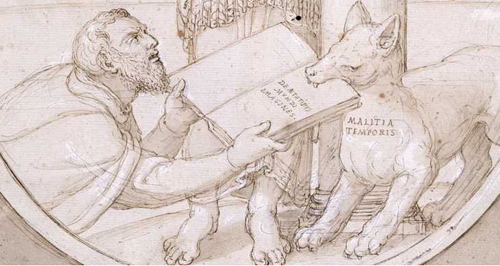
\includegraphics[height=0.3\textheight,keepaspectratio]
                          {images/malatia-temporis.png}
  \caption{Pormenor de um desenho de Franscisco da Holanda, ``O
    artista apresentando o seu livro''}
  \label{fig:1}
\end{figure}

Já para as campanhas em África, D. Sebastião viria a escolher outros %
engenheiros para o acompanharem \cite[notas,p.54]{holanda} e
perder-se-ia em Alcácer-Quibir, vítima certamente de uma campanha mal
desenhada. É portanto pouco provável que estes apelos tenham sido
ouvido pelo seu destinatário. A propósito, Jorge Segurado observa
\cite{segurado}.

\begin{quote}
  Desde o seu queixume a D. Sebastião, no seu tratado em 1571, até à
  morte do Arquitecto, em 1584, decorreram cerca de treze anos, final
  amargo e triste para o mais importante artista da Renascença em
  Portugal.
\end{quote}

Por volta de 1573, dois anos depois de terminar ``A Ciência do
Desenho'', Franscisco d'Holanda desenha um insólito auto-retrato
(Figura \ref{fig:1}) para o seu ``Livro das Idades''. Este livro
acompanhou-o durante praticamente toda a vida e Felipe II, que o
artista terá ainda visto sentar-se no trono português, viria a levá-lo
para o Escorial de Madrid. No desenho, o artista apresenta o seu livro
a um cão que o morde furiosamente. No peito do cão lê-se a inscrição
``malatia temporis''.

\printbibliography[heading=bibliography,title={Bibliografia}]

\end{document}
